\makeatletter
\def\input@path{{../../}}
\makeatother
\documentclass[../../main.tex]{subfiles}
\graphicspath{
	{../../img/}
	{../img/}
	{img/}
}

\begin{document}
В общем случае, если имеется окружность радиуса $R$ с центром в точке $O$ и
две точки $M$ и $N$ ($M$~--- внутри, а $N$~--- вне окружности) то, проводя 
луч $OMN$, говорят, что точки $M$ и $N$ находятся в 
\emph{инверсии (симметрии)} отностительно
рассматриваемой окружности, если $OM \cdot ON = R^2$.

Для простейшего дробно-линейного отображения $ w = \dfrac{1}{z}$  имеем: 
$ |w| = \dfrac{1}{|z|} \implies {|z| \cdot |w| = 1}$, т.~е. преобразование $z$
из плоскости \textcircled{$z$}  и образ $w$ в  \textcircled{$w$} будут
находиться в инверсии относительно окружности с $R  = 1$.

\begin{erem}
 Википедия утверждает, что в комплексной плоскости инверсия~--- это
 $\dfrac 1{\overline z}$, а не $\dfrac 1z$
 (используется $\overline{z}$ вместо $z$).
\end{erem}

\begin{center}
	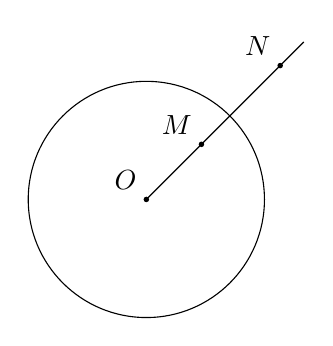
\begin{tikzpicture}
    \draw[color=black] (0,0) circle(1.5);
    \fill(0,0) circle(1pt) node[above left] {$O$};
    \fill(0.7,0.7) circle(1pt) node[above left] {$M$};
    \fill(1.7,1.7) circle(1pt) node[above left] {$N$};
    \draw (0,0) -- (2,2);
	\end{tikzpicture}
	\begin{tikzpicture}
	\draw[->] (-2.5,0) -- (2.5,0);
	\draw[->] (0,-2.5) -- (0,2.5) node[below right] {\textcircled{$z$}};
    \draw[loosely dashed] (0,0) circle(1.5);
    \draw(1.5, -0.1) node[below left]{$1$}-- (1.5, 0.1);
    \draw(-1.5, -0.1) node[below left]{$-1$} -- (-1.5, 0.1);
    \fill(0.6,0.6) circle(1pt) node[above left] {$Z$};
	\end{tikzpicture}
	\begin{tikzpicture}
	\draw[->] (-2.5,0) -- (2.5,0);
	\draw[->] (0,-2.5) -- (0,2.5) node[below right] {\textcircled{$w$}};
    \draw[loosely dashed] (0,0) circle(1.5);
    \draw(1.5, -0.1) node[below left]{$1$}-- (1.5, 0.1);
    \draw(-1.5, -0.1) node[below left]{$-1$} -- (-1.5, 0.1);
    \fill(0,0) circle(1pt) node[above left] {$O$};
    \fill(0.7,0.7) circle(1pt) node[above left] {$M$};
    \fill(1.7,1.7) circle(1pt) node[above left] {$N$};
    \draw (1.9,1.5) node[right]  {$w = \frac{1}{z}$};
    \draw (2,0.6) node[right]  {$OM \cdot ON = 1$};
    \draw (0,0) -- (2,2);
	\end{tikzpicture}
\end{center}
В дальнейшем под \emph{окружностью (прямой)} на комплексной плоскости в 
широком смысле слова будем
подразумевать, как окружность, так и прямую.
В соответствии с этим общее дробно-линейное пребразование обладает следующим
свойством: окружность при дробно-линейном преобразовании переходит либо
в окружность, либо в прямую, а прямая может перейти как
в прямую, так и в окружность.

Т.~к. линейное отображение
является частным случаем дробно-линейного, то для него существует
похожее свойство: прямая переходит только в прямую,
окружность~--- только в окружность.

Если в плоскости \textcircled{$z$} заданы различные точки $z_1, z_2, z_3$,
переходящие при соответствующем дробно-линейном преобразовании 
\eqref{lec25:7} последовательно в точки $w_1, w_2, w_3$ в 
\textcircled{$w$}, то можно показать, что \eqref{lec25:7} в этом случае
удовлетворяет условию:
\begin{equation}
\label{lec26:1} \frac{w - w_1}{w - w_2} \cdot \frac{w_3 - w_2}{w_3 - w_1} = 
\frac{z - z_1}{z - z_2} \cdot \frac{z_3 - z_2}{z_3 - z_1}.
\end{equation}

В случае работы в рассматриваемой комплексной плоскости (КП), если в 
\eqref{lec26:1} одна из точек
$z_k ,\ k = \overline{1,3}$ или $w_k ,\ k = \overline{1,3}$ равна 
$\infty$, то тогда все разности в \eqref{lec26:1}, использующие 
эти точки, заменяют на $1$.

Например, если $z_3 = \infty$ переходит в $w_3 \neq \infty$, то тогда 
\eqref{lec26:1} записывается в виде
\[
\frac{w - w_1}{w - w_2} \cdot \frac{w_3 - w_2}{w_3 - w_1} = 
\frac{z - z_1}{z - z_2}.
\]
Аналогично, если 
$z_3 = \infty \underset{\text{переходит в}}{\rightarrowtail} w_3 = \infty$, то
\[
\frac{w - w_1}{w - w_2} = \frac{z - z_1}{z - z_2}.
\]

\begin{examples}
\;

 \begin{enumerate}
  \item
 Найдём дробно-линейное преобразование \eqref{lec25:7}, 
 для которого
 \[
 \begin{cases}
w(1) = i \\ 
w(0) = 2 \\
w(-i) = 1  
 \end{cases}
\]
 \[\begin{cases}
  z_1 = 1 \rightarrowtail w_1 = i \\
  z_2 = 0 \rightarrowtail w_1 = 2 \\
  z_3 = -i \rightarrowtail w_1 = 1 \\
  \end{cases}
 \]
 Т.~к. $z_1, z_2, z_3$ не лежат на одной прямой в \textcircled{$z$}, 
 а $w_1, w_2, w_3$ также не лежат на одной прямой в \textcircled{$w$}, 
 получаем, что окружность плоскости \textcircled{$z$} проходящая через
 $z_1, z_2, z_3$  перейдёт в соответствующую окружность \textcircled{$w$},
 проходящую через $w_1, w_2, w_3$. В силу \eqref{lec26:1}:
 \[
  \frac{1 - 2}{1 - i} \cdot \frac{w - i}{w - 2} = 
  \frac{z - 1}{z - 0} \cdot \frac{-i - 0}{-i - 1} =
  \frac{z - 1}{z} \cdot \frac{1}{1 - i}
 \]
 \[
  -\frac{w - i}{w - 2} = \frac{z - 1}{z}
 \]
 \[
  -zw +iz = (z - 1)(w - 2) = zw - 2z - w + 2
 \]
 \[
  (2z - 1)w = (2 + i)z - 2
 \]
 \[
  w = \frac{(2 + i)z - 2}{2z - 1}
 \]
При этом $z= \frac{1}{2} \rightarrowtail w = \infty$, поэтому если если в $
\textcircled{z}$ есть окружность, проходящая через три различные точки, одна 
из которых~--- $\frac{1}{2}$, то она в $\textcircled{w}$ перейдет в 
окружность в широком смысле, т.~е. в прямую.
\item
\[
 \begin{cases}
  w(0) = \infty\\
  w(\infty) = i\\
  w(1 + i) = 1 + i
 \end{cases}
\]
В этом случаем в силу \eqref{lec26:1} имеем:
\[
  \begin{cases}
  w(0) = \infty\\
  w(\infty) = i\\
  w(1 + i) = 1 + i
 \end{cases}
 \implies \frac{w_3 - w_2}{w - w_2} = \frac{z - z_1}{z_3 - z_1}
\]
\[
 \frac{1 + i - i}{w - i} = \frac{z - 0}{1 + i - 0} \implies
 w - i = \frac{1 + i}{z} \iff w = \frac{1 + i}{z} + i.
\]
Можно показать, что имеют место следующие частные случаи 
дробно-линейных отображений:
\begin{enumerate}
 \item 
 \[
  \begin{cases}
   w = A\cdot \dfrac{z - z_1}{z - z_2},\\
   A \in \C,
  \end{cases}\]
при этом
$\begin{cases}
  z_1 \rightarrowtail 0,\\
  z_2 \rightarrowtail \infty.  
 \end{cases}
 $
Если окружность (прямая) содержит точку $z_2$, то при рассмотрении отображения
её образом будет прямая, иначе~--- окружность.
 \item
\[
\begin{cases}
 w = e^{i\alpha} \dfrac{z - z_0}{z- \overline{z_0}}, \\
 \alpha \in \R,\  \Im z_0 > 0.
\end{cases}     
\]
При этом отображении мнимая полуплоскость $\Im z_0 > 0$ в \textcircled{$z$} 
переходит в единичный круг $|w| < 1$ в \textcircled{$w$} так,
что $z_0$ из \textcircled{$z$} переходит в центр круга в плоскости
\textcircled{$w$}.

 \item
\[
 \begin{cases}
  w = e^{i\alpha} \dfrac{z - z_0}{1 - z \overline{z_0}}, \\
  \alpha \in \R.
 \end{cases}
\]
При этом отображении единичный круг в плоскости \textcircled{$z$}
переходит в единичный круг \textcircled{$w$} так, что точка $z_0$ переходит
в центр круга  $w_0 = 0$ в плоскости \textcircled{$w$}.
\end{enumerate}

\end{enumerate}
\end{examples}

\subsection{Степенная ФКП с натуральным показателем и обратная к ней ФКП}
Рассмотрим
\begin{equation}
\label{lec26:2}
\begin{cases}
 w = f(z) = z^n \\
 n \in \N
\end{cases}
\end{equation}

Если $n = 1$, то $w \stackrel{\eqref{lec26:2}}{=} z$ ~-- 
идентичное ФКП (идентичное отображение).
При этом отображении преобразование плоскости \textcircled{$z$} 
даёт такой же образ в \textcircled{$w$}.

Пусть $n \geq 2$.
\[
\begin{cases}
 z =re^{i\phi}\\
 r = |z| \\
 \phi = \arg z \in \left] -\pi, \pi \right] \implies &
\end{cases}
\implies
\begin{cases}
 w\stackrel{\eqref{lec26:2}}{=} r^ne^{in\phi} \\
|w| = r^{n} \\
\Arg w = n \phi + 2\pi k, k \in \Z
\end{cases}
\]

Рассмотрим частный случай $n = 2$, т.~е. $w = z^2 = r^2e^{2i\phi}$.
\[
 \begin{cases}
  |w| = r^2 \\
\Arg w = 2\phi + 2\pi k, k \in X
 \end{cases}
\]
\begin{enumerate}
\item
\[
0 < \arg z < \frac{\pi}{2} \implies 
0 < \arg w < \pi
\]
I четверть \textcircled{$z$} $\rightarrowtail$ 
верхняя полуплоскость плоскости \textcircled{$w$}.
\begin{center}
	\begin{tikzpicture}
	\draw[->] (-2.5,0) -- (2.5,0);
	\draw[->] (0,-2.5) -- (0,2.5) node[above right] {\textcircled{$z$}};
	
    \pattern[pattern=north east lines] 
    (0.3,0.3)--(0.3,2.5)--(2.5,2.5)--(2.5,0.3)--cycle;
    \draw[dashed] (0.3,0.3) -- (0.3,2.5);
    \draw[dashed] (0.3,0.3) -- (2.5,0.3);
	
    \draw[->] (4.5,0) -- (9.5,0);
	\draw[->] (7,-2.5) -- (7,2.5) node[above right] {\textcircled{$w$}};
	
    \pattern[pattern=north east lines] 
    (4.5,0.3)--(9.5,0.3)--(9.5,2.5)--(4.5,2.5)--cycle;
    \draw[dashed] (4.5,0.3) -- (9.5,0.3);
    
    \draw[->, thick] (2.6,2) .. controls (3.5,2.5) .. (4.4, 2)
    node[pos=0.6,above]{$w = z^2$};
	\end{tikzpicture}
\end{center}

\item
\[
 0 < \arg z < \pi \implies 0 < \arg w < 2\pi
\]
В данном случае верхняя полуплоскость \textcircled{$z$}
отображается во всю плоскость  \textcircled{$w$}
c разделением вдоль положительной части действительной оси.

\begin{center}
	\begin{tikzpicture}
	\draw[->] (-2.5,0) -- (2.5,0);
	\draw[->] (0,-2.5) -- (0,2.5) node[above right] {\textcircled{$z$}};
	
    \pattern[pattern=north east lines]
    (-2.5,0.3)--(-2.5,2.5)--(2.5,2.5)--(2.5,0.3)--cycle;
    \draw[dashed] (-2.5,0.3) -- (2.5,0.3);
	
    \draw[->] (4.5,0) -- (9.5,0);
	\draw[->] (7,-2.5) -- (7,2.5) node[above right] {\textcircled{$w$}};
	
    \pattern[pattern=north east lines]
    (4.5,0.3)--(9.5,0.3)--(9.5,2.5)--(4.5,2.5)--cycle;
    \draw[dashed] (4.5,0.3) -- (9.5,0.3);
    \pattern[pattern=north east lines]
    (4.5,-0.3)--(9.5,-0.3)--(9.5,-2.5)--(4.5,-2.5)--cycle;
    \draw[dashed] (4.5, -0.3) -- (9.5, -0.3);
    
    \draw[->, thick] (2.6,2) .. controls (3.5,2.5) .. (4.4, 2)
    node[pos=0.6,above]{$w = z^2$};
	\end{tikzpicture}
\end{center}
\end{enumerate}

Аналогично поступают и в случаях: $n > 2,\ n \in \N$.
Обратную к степенной функции с натуральным показателем $n \in \N: w^n = z$
определяют как решение уравнения
\[w = {|z|}^{\textstyle \frac{1}{n}}e^{i\frac{\arg z + 2 \pi k}{n}}.\]
Имеем многозначность. В этом случае, если придавать $k \in \Z$ последовательно
значения, то каждое из них будет давать одну из ветвей рассмотренной
многозначной ФКП. На практике для определения ветви рассматривают 
соответствующие начальные условия 
${z_0 \neq 0}$. Рассматривая $\sqrt[n]{z_0} = {|z|}^{\frac{1}{n}}e^{i
\frac{\phi + 2 \pi m}{n}},\ m \in \Z$, по значению 
$\sqrt[n]{z_0}$ однозначно определяют $m \in \Z$. Тогда для найденного 
$m=k$ получаем, что $w = \sqrt[n]{z} = |z|^{\textstyle 
\frac{1}{n}} e^{i \frac{\phi_0 + 2 \pi k}{n}}$.

\begin{example}
 Рассмотрим ветвь $\sqrt[3]{z}$, для которой 
 $\sqrt[3]{i} = e ^{\textstyle \frac{\pi i}{6}}$. В данном случае для 
 $z_0 = i$ получаем \[z_0 = |z_0| e^{\textstyle i(\phi_0 + 2 \pi k)} = 
 e^{\textstyle i(\frac{\pi}{2} + 2 \pi k)} \implies \sqrt[3]{z} = 
 \left(e^{\textstyle i(\frac{\pi}{2} + 2 \pi k)}\right)^{\textstyle 
 \frac{1}{3}} =
 e^{\textstyle i(\frac{\pi}{6} + \frac{2 \pi k}{3})}.\]
 Т.~к. в силу начального условия 
 $\sqrt[3]{i} = e ^{\textstyle i \frac{\pi}{6}}$, то тогда
 берем ветвь $k = 0$, 
 поэтому в данном случае \[w = \sqrt[3]{z}
 = {|z|}^{\tfrac{1}{3}}e ^{\textstyle i( \frac{\pi}{6} + 0)}
 = {|z|}^{\tfrac{1}{3}}e ^{\textstyle i( \frac{\pi}{6})} 
 = \frac{\sqrt{3} + i }{2} \sqrt[3]{|z|}.\]
\end{example}

\subsection{Комплексная экпонента. Гиперболические и тригонометрические ФКП}
Для 
$
\begin{cases}
 z = x + iy \\
 x, y \in \R
\end{cases}
$
по определению считают $\exp z = e^x(\cos y  + i \sin y) $.

Если $y = \Im z = 0$, то $z = x \in \R$, т.~е.
$\exp z = e^x$.
В связи с этим также в общем случае будем использовать
\begin{equation}
\label{lec26:3}
 \exp z = e^z = e^{x + iy} = e^{x}(\cos y + i \sin y).
\end{equation}
В силу \eqref{lec26:3}, используя соответствующие свойства действительных 
тригонометрических и экспоненциальных функций, имеем:
 \begin{enumerate}
    \item $e^0 = 1$
    \item $e^{z_1} \cdot e^{z_2} = e^{z_1 + z_2},\ \forall z_1, z_2 \in \C$
    \item $\dfrac{e^{z_1}}{e^{z_2}} = e^{z_1 - z_2},\ \forall z_1, z_2 \in \C$
 \end{enumerate}
В отличии от действительной экспоненты, комплексная экспонента \eqref{lec26:3} 
будет 
периодической с основным периодом $T_0 = 2\pi i$, т.~к.
\[\forall k \in \Z \implies e^{z + kT_0} = e^{z + 2 \pi k i} 
= e^{z} e^{2 \pi k i} = e^z(\cos{2 \pi k} + i \sin{2 \pi k}) = e^z.\]

С помощью \eqref{lec26:3} определяют гиперболические ФКП:
\[
 \ch{z} = \frac{e^z + e^{-z}}{2}
\]
\[
 \sh{z} = \frac{e^z - e^{-z}}{2}
\]
\[
 \th{z} = \frac{\sh{z}}{\ch{z}} = \frac{e^{2z} - 1}{e^{2z} + 1},\ 
 z \neq i\left(\frac{\pi}{2} + \pi k\right),\ k \in \Z
\]
\[
 \cth{z} = \frac{\ch{z}}{\sh{z}} =
 \frac{e^{2z} + 1}{e^{2z} - 1},\ z \neq i \pi k,\ k \in \Z
\]
Для гиперболической ФКП сохраняются все свойства действительных 
гиперболических функций.
Например:
\begin{enumerate}
 \item $\ch^{2}{z} - \sh^{2}{z} = 1$~--- основное гиперболическое тождество;
 \item $1 - \th^{2}{z} = \dfrac{1}{\ch^{2}{z}}$;
 \item $\cth^{2}{z} - 1= \dfrac{1}{\sh^{2}{z}}$;
 \item $\sh{2z} = 2\sh{z} \ch{z}$;
 \item $\ch{2z} = \ch^{2}{z} + \sh^{2}{z}$.
\end{enumerate}

Теперь введем тригонометрические ФКП.
При этом, в отличие от вещественных синуса и косинуса, которые являются 
ограниченными функциями, вводимые тригонометрические ФКП не являются 
ограниченными.

Полагаем
\[\cos{z} = \frac{e^{iz} + e^{-iz}}{2} = \ch{iz}\]
\[
 \sin{z} = \frac{e^{iz} - e^{-iz}}{2i} = -i \sh{iz}
\]
\[
 \tg{z} = \frac{\sin{z}}{\cos{z}},\ z \neq \frac{\pi}{2} + k,\ k \in \Z
\]
\[
 \ctg{z} = \frac{\cos{z}}{\sin{z}},\ z \neq \pi k,\ k \in \Z
\]
Нетрудно видеть, что
\[\tg{z} = -i\th{iz},\]
\[\ctg{z} = i\cth{iz},\]
а также, как и для действительных тригонометрических функций, выполняется:
\begin{enumerate}
\item $\cos^2{z} + \sin^2{z} = 1\text{~--- основное тригонометрическое 
тождество}$;
\item $1 + \tg^{2}{z} = \dfrac{1}{\cos^2{z}}$;
\item $1 + \ctg^{2}{z} = \dfrac{1}{\sin^2{z}}$;
\item $\sin{2z} = 2 \sin{z} \cos{z}$;
\item $\cos{2z} = \cos^{2}{z} -  \sin^{2}{z}$.
\end{enumerate}

Хотя для тригонометрических ФКП выполняется основное тригонометрическое
тождество, из него уже не следует ограниченность 
тригонометрической ФКП.

\subsection{Логарифмическая ФКП}
Логарифмическая ФКП обозначается $w = \Ln{z}$ 
и определяется как решение уравнения 
\begin{equation}
 \label{lec26;4}
 \begin{cases}
   e^{w} = z, \\
   z \neq 0.
 \end{cases}
\end{equation}

\end{document}
